\scanpage{158}
% archive foliation: 157

\deleted{$\unsure{IV''_5}$} $V''_4$ \deleted{Avenir-passé} \unsure{Durée}

\begin{center}
\begin{tabular}{rcl}
A v e n i r & -- & p a s s é\\
destinée & -- & histoire\\
pérennité & -- & ancienneté\\
innovation & -- & tradition (III)\\
\deleted{le nouveau} & \deleted{--} & \deleted{l'ancien}\\
\multicolumn{3}{l}{\deleted{\illegible{4}}}\\
élan & -- & enracinement (II)
\end{tabular}
\end{center}

\deleted{$\unsure{IV''_6}$} $V''_5$ Espace-temps

\begin{center}
\begin{tabular}{rcl}
E s p a c e & -- & t e m p s\\
étendue (ou distance) & -- & durée\\
\deleted{ubiquité} & \deleted{--} & \deleted{éternité}
\end{tabular}
\end{center}

\margin{$\unsure{=\ ?\ ?}$}
\figure{\begin{tikzpicture}[x=1cm,y=1cm]
\draw (0,0)--(1.4,4.7);
\end{tikzpicture}}
\margin{\(\left\{\begin{array}{l}
\text{Complément t. d. m.}\quad\text{(+ harmonie)}\\
\text{mise en page liste}\\
\text{\unsure{fenêtre carrée}}\\
\text{dessins \ldots}
\end{array}\right.\)}

98 \quad (*) texte barré

\deleted{\unsure{99}} \quad (**) Plusieurs existences successives

100 \quad (*) texte barré

(**) Elle qui n'a point lu. Comparer note n° 162; \unsure{p. dep.} (\unsure{a}) p. \unsure{789}
``conviction et connaissance''

\figure{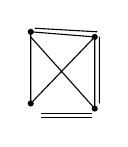
\begin{tikzpicture}[scale=.65]
\draw (0,0)--(0,1.4)--(1.25,1.3)--(1.25,-.1);
\draw (0,0)--(1.25,1.3) (0,1.3)--(1.25,-.1);
\draw (.2,-.2)--(1.2,-.2) (.2,-.28)--(1.2,-.28);
\draw (.08,1.47)--(1.3,1.4) (1.34,1.3)--(1.34,0);
\foreach \p in {(0,0),(0,1.4),(1.25,1.3),(1.25,-.1)}\fill \p circle(.06);
\end{tikzpicture}}

(***) \unsure{Ref. aux} 1977. Frustration.

103 \quad (*) Autre \unsure{perspective}.

107 \quad (*) Mais pas \unsure{assez} pour la multiplication.

(**) \unsure{Copie d'élève}

(***) \unsure{cheminement} \illegible{1} \unsure{logique}.

110 \quad \unsure{Pensée} par \unsure{réciprocité}

\figure{\begin{tikzpicture}[x=.7cm,y=.7cm]
% Upper left pair of joined figures.
\coordinate (A) at (2,10);\coordinate (B) at (2.8,10.8);\coordinate (C) at (3.3,10);
\coordinate (D) at (1.3,7.8);\coordinate (E) at (3.2,8.1);\coordinate (F) at (2.3,8.8);
\draw[very thick] (A)--(B);\draw (A)--(C)--(B) (A)--(D)--(E)--(A) (D)--(F)--(A) (F)--(E);
\draw (1.25,7.7) .. controls (1.3,9) and (1.6,9.7) .. (A);
\foreach \p in {A,B,C}\fill (\p) circle(.05);
% Left-hand small fan and joined tetrahedral forms.
\draw (.5,8.7)--(-.6,8.1)--(.35,7.65);
\draw[very thick] (-.6,8.1) .. controls (-.1,8.05) and (.25,7.8) .. (.35,7.65);
\draw (.35,7.65)--(.05,6.4)--(1.05,6.15)--(1.45,6.95)--cycle;
\draw (.35,7.65)--(1.05,6.15) (.05,6.4)--(1.45,6.95) (.35,7.65)--(.8,6.85)--(.05,6.4) (.8,6.85)--(1.05,6.15);
\draw[very thick] (.35,7.65)--(.8,6.85);
% Middle-left diamond.
\coordinate (a) at (4,7.6);\coordinate (b) at (3,5.95);\coordinate (c) at (5.1,5.9);\coordinate (d) at (4.65,4.55);
\draw (a)--(b)--(d)--(c)--cycle (a)--(d) (b)--(c);
\draw (b) .. controls (4,6.2) and (4.6,6.1) .. (c);
\draw[very thick] (a)--(c) (c)--(d) (a)--(d);
\fill (b) circle(.06);\draw (c) circle(.1);
\node[above] at (a) {$a$};\node[left] at (b) {$b$};
% Heavily retraced central complex.
\coordinate (p) at (8.2,8.05);\coordinate (q) at (10.1,8.6);\coordinate (r) at (9.35,7.5);
\coordinate (s) at (8.7,6.35);\coordinate (t) at (10,6.25);\coordinate (u) at (9.6,5.2);
\draw[line width=2pt] (p)--(q)--(r)--cycle (p)--(s)--(t)--(r)--(s) (s)--(u)--(t);
\draw (p)--(t) (r)--(u) (s)--(q);
\foreach \x in {8.55,8.7,8.85,9,9.15}\draw (\x,7.8)--(\x+.25,7.45);
\foreach \x in {9.25,9.4,9.55,9.7}\draw (\x,7.15)--(\x-.05,6.35);
\foreach \x in {9,9.15,9.3,9.45,9.6,9.75}\draw (\x,6.25)--(9.6,5.3);
\draw (9.3,5.05)--(10.6,5.05) (9.3,4.98)--(10.6,4.98);
\node[above left] at (p) {$c'$};\node[above] at (q) {$\unsure{v}$};\node[left] at (r) {$a$};
\node[left] at (s) {$b$};\node[right] at (t) {$c$};\node[below] at (u) {$u$};
\node at (10.5,5.2) {$\deleted{\unsure{u}}$};
% Lists to the right of the complex.
\node[draw,ellipse,inner sep=2pt] at (12.15,9.4) {$abc$};
\node at (12.15,8.7) {$bcu$};
\node at (12.15,8) {$acu$};\draw (11.9,8) ellipse(.4 and .25);
\node at (12.15,7.3) {$abc'$};
\node at (13.1,6.6) {$\unsure{c'au}\quad\text{ou}\quad c'av$};
\node at (13.1,5.9) {$\unsure{c'bu}\quad\text{ou}\quad c'bv$};
\node[align=left] at (15,9.1) {$ac$\\$bc$\\$ab$\\$c'a$\\$c'b'$};
% Lower left figure and hatched quadrilateral.
\draw (.1,4.2)--(.3,2.9)--(1.8,2.8)--(1,1.9)--cycle;
\draw (.3,2.9)--(1.15,4.1)--(1.8,2.8) (1.15,4.1)--(1,1.9);
\draw (-.1,4.5)--(1,4.3) (-.1,4.5)--(.1,3.1);
\foreach \x in {.1,.25,.4,.55,.7}\draw (\x,4.35)--(\x+.12,3.35);
\foreach \x in {.65,.8,.95,1.1,1.25}\draw (\x,3.15)--(1.25,3.8);
\draw (.4,2.8)--(1,2.15) (.6,2.8)--(1.3,2.5);
% Long diamond at the bottom.
\coordinate (h) at (6.6,4.15);\coordinate (i) at (6.05,1.65);\coordinate (j) at (7.35,1.7);\coordinate (k) at (6.9,-.85);\coordinate (l) at (6.95,.3);
\draw (h)--(i)--(k)--(j)--cycle (i)--(j) (h)--(l) (i)--(l)--(j);
\draw (i) .. controls (6.25,.6) and (6.65,-.9) .. (k) (j) .. controls (7.5,.4) and (7.3,-.6) .. (k);
\foreach \x in {6.48,6.56,6.64,6.72}\draw (\x,3.1)--(\x+.24,3.5);
\node[left] at (i) {$a$};\node[right] at (j) {$b$};\node[above] at (k) {$\unsure{c}$};
% Lower middle-right bent figure.
\draw (10.2,4.05)--(10.9,3.65)--(11.65,2.3)--(11,1.25)--cycle (10.2,4.05)--(10.6,2.6)--(11.65,2.3) (10.6,2.6)--(11,1.25) (10.9,3.65)--(11,1.25);
\draw (9.95,3.2)--(9.95,4.2)--(10.2,4.05);
\foreach \x in {10.35,10.5,10.65,10.8,10.95}\draw (\x,3.6)--(\x-.1,2.7);
% Isolated triangular stroke and small right diamond.
\draw (14.1,4.15)--(14.65,3.2) (14.1,4.15)--(14.1,2.35)--(14.65,3.15);
\node at (13.8,2.85) {$*$};
\draw (16.8,4.9)--(16.15,4.1)--(16.6,3)--(17.15,4.05)--cycle (16.15,4.1)--(17.15,4.05) (16.8,4.9)--(16.6,3);
\foreach \x in {16.35,16.5,16.65}\draw (\x,4.15)--(16.8,4.8);
\draw (16.35,3.65)--(16.6,4) (16.5,3.4)--(16.8,4);
\end{tikzpicture}}
